% !TEX program = lualatex
\documentclass[final]{beamer}

% ====================
% Pacotes
% ====================

\usepackage[T1]{fontenc}
\usepackage{lmodern}
\usepackage[orientation=portrait,size=a0,scale=1.2]{beamerposter}
\usepackage[portuguese]{babel}
\usepackage{amsmath, amssymb}
\usepackage{graphicx}
\usepackage{booktabs}

\usetheme{gemini}
\usecolortheme{labfluid}

% ====================
% Configurações de Layout
% ====================

\newlength{\sepwidth}
\newlength{\colwidth}
\setlength{\sepwidth}{0.04\paperwidth}
\setlength{\colwidth}{0.44\paperwidth}

\newcommand{\separatorcolumn}{\begin{column}{\sepwidth}\end{column}}

% ====================
% Informações do Cabeçalho
% ====================

\title{Inteligência Artificial na Solução Numérica de Equações Diferenciais Parciais Não Lineares}
\author{Samuel Kutz Paranhos \\[1ex] Prof. Roberto Ribeiro \\[4ex]}
\institute{\normalsize PIBIC 2024}



\setlength{\fboxsep}{8pt} % Adiciona um "padding" à caixa branca

% Ajuste das Logos Laterais
\logoleft{%
  % O [s] no final permite que o \vfill distribua o espaço verticalmente
  \begin{minipage}[c][16cm][s]{15cm} 
    \centering
    % Logo Superior Esquerda
    
\includegraphics[height=8cm,keepaspectratio]{imgs/brasao_UFSC.png}
    \vfill % Isso empurra a próxima imagem para o fundo
    
    % Logo Inferior Esquerda
    
\includegraphics[height=11cm,keepaspectratio]{imgs/BrazOpt_LOGO.png}
  \end{minipage}
}

\logoright{%
  \begin{minipage}[c][16cm][s]{15cm}
    \centering
    % Logo Superior Direita
    
\includegraphics[height=11cm,keepaspectratio]{imgs/LabFluidLogo.png}
    %\vfill % Isso empurra a próxima imagem para o fundo
    
    \vspace{1.75cm}

    % Logo Inferior Direita
    
\includegraphics[height=3cm,keepaspectratio]{imgs/CNPq.png}
  \end{minipage}
}

% ====================
% Início do Documento
% ====================

\begin{document}


\begin{frame}[t]
\begin{columns}[t]
\separatorcolumn

% --------------------
% --- COLUNA 1 -------
% --------------------
\begin{column}{\colwidth}

  \begin{block}{Introdução}
    Este trabalho investiga as \textcolor{UniBlue}{Redes Neurais Fisicamente Guiadas (PINNs)}, uma alternativa baseada em \textit{Deep Learning} que aproxima soluções de Equações Diferenciais Parciais (EDPs) de forma contínua, incorporando a EDP diretamente na função de perda da rede neural durante seu treinamento \cite{raissi2017}, como um termo de regularização.

    O objetivo é, portanto, averiguar a performance desta abordagem na solução do sistema de Boussinesq, um modelo não linear para a simulação de ondas aquáticas.
  \end{block}

  \begin{block}{Physics-Informed Neural Networks (PINNs)}
    As PINNs adaptam a arquitetura de redes neurais (neste caso, são \textit{Multilayer Perceptrons}, MLPs) para encontrar soluções aproximadas de instâncias de EDPs. O método visa solucionar um sistema genérico, escrito em termos de um operador diferencial $\mathcal{D}$:
    \begin{equation*}
        \left\{
        \begin{aligned}
            & \mathcal{D}[u](x,t) = 0, \quad \forall (x,t) \in \Omega \times (0, T] \\
            & u(x,0) = u_0(x), \quad x \in \Omega
        \end{aligned}
        \right.
    \end{equation*}
    A rede é treinada para minimizar o Erro Quadrático Médio (EQM), combinando os erros da física e das condições iniciais:
    \begin{equation*}
    \resizebox{0.9\columnwidth}{!}{ $
    \text{EQM}(\theta) = \underbrace{\frac{1}{N_{\mathcal{D}}} \sum_{i=1}^{N_{\mathcal{D}}} \left( \mathcal{D}[u_\theta](x_i, t_i) \right)^2}_{\text{Resíduo da EDP}} +
                       \underbrace{\frac{1}{N_{0}} \sum_{j=1}^{N_{0}} \left( u_\theta(x_j, 0) - u_0(x_j) \right)^2}_{\text{Cond. Inicial}}
    $ }
    \end{equation*}
    onde $\{x_i, t_i\}_{i=1}^{N_{\mathcal{D}}}$ são os pontos de colocação no interior do domínio e $\{x_j\}_{j=1}^{N_0}$ são os pontos de colocação amostrados na condição inicial. Estes pontos são, usualmente, amostrados por distribuições uniformes ao longo do domínio da EDP.
  \end{block}
  \begin{block}{O Sistema de Boussinesq}
    Este sistema descreve a propagação de ondas em águas rasas, modelando a evolução da elevação da superfície, $\eta(x,t)$, e da média vertical da velocidade horizontal, $u(x,t)$: 
    \begin{equation*}
    \left\{
    \begin{aligned}
        & \eta_t + u_x + \alpha(\eta u)_x = 0, \qquad \text{para } (x,t) \in [-30, 30] \times [0, 15] \\
        & u_t + \eta_x + \alpha u u_x - \tfrac{\beta}{3} u_{xxt} = 0, \\
        % & \eta(x, 0) = \text{sech}^2(x), \\
        % & u(x, 0) = 0.
    \end{aligned}
    \right.
    \end{equation*}
    onde $\alpha$ e $\beta$ são parâmetros que controlam os efeitos de não linearidade e dispersão. No nosso estudo, resolvemos este problema sujeito à condição inicial
    \begin{equation*}
    \begin{aligned}
        & \eta(x, 0) = \text{sech}^2(x), \\
        & u(x, 0) = 0.
    \end{aligned}
    \end{equation*}

    Estas condições iniciais são escolhidas porque no caso em que $\alpha = \beta = 0$, a solução desse problema pode ser determinada de forma exata pela fórmula de D'Alambert, tornando-o um bom teste para PINNs. No caso contrário, a eficácia será testada comparando com a solução proveniente do método pseudoespectral.
  \end{block}
  
  \begin{block}{Viés Espectral e Amostragem Adaptativa}
    Uma dificuldade conhecida em PINNs é o Viés Espectral \cite{rahaman2019spectral}, uma tendência de redes neurais MLPs em aprender primeiro as componentes de baixa frequência da solução. A fim de mitigar este efeito, implementa-se a amostragem adaptativa \textit{Residual-based Adaptive Refinement} (RAR) \cite{wu2023comprehensive}, que consiste em abandonar a distribuição uniforme de pontos e amostrar novos pontos com base em uma densidade de probabilidade $p(x)$ que prioriza regiões de maior erro (resíduo da EDP, $\epsilon(x) = |\mathcal{D}[u_\theta](x,t)|$). 
    
    Em RAR, para $ k, c \geq 0 $, a função densidade de probabilidade é da forma (sujeito a normalização):
    \begin{equation*}
        p(x) \propto \frac{|\epsilon(x)|^k}{\mathbb{E}[|\epsilon(x)|^k]} + c.
    \end{equation*}
   Isso leva a rede a priorizar a alocação de pontos onde o resíduo está sendo maior (onde está errando mais), como visualizado na Figura \ref{fig:sampling_dist}.
    \begin{figure}
        \centering
        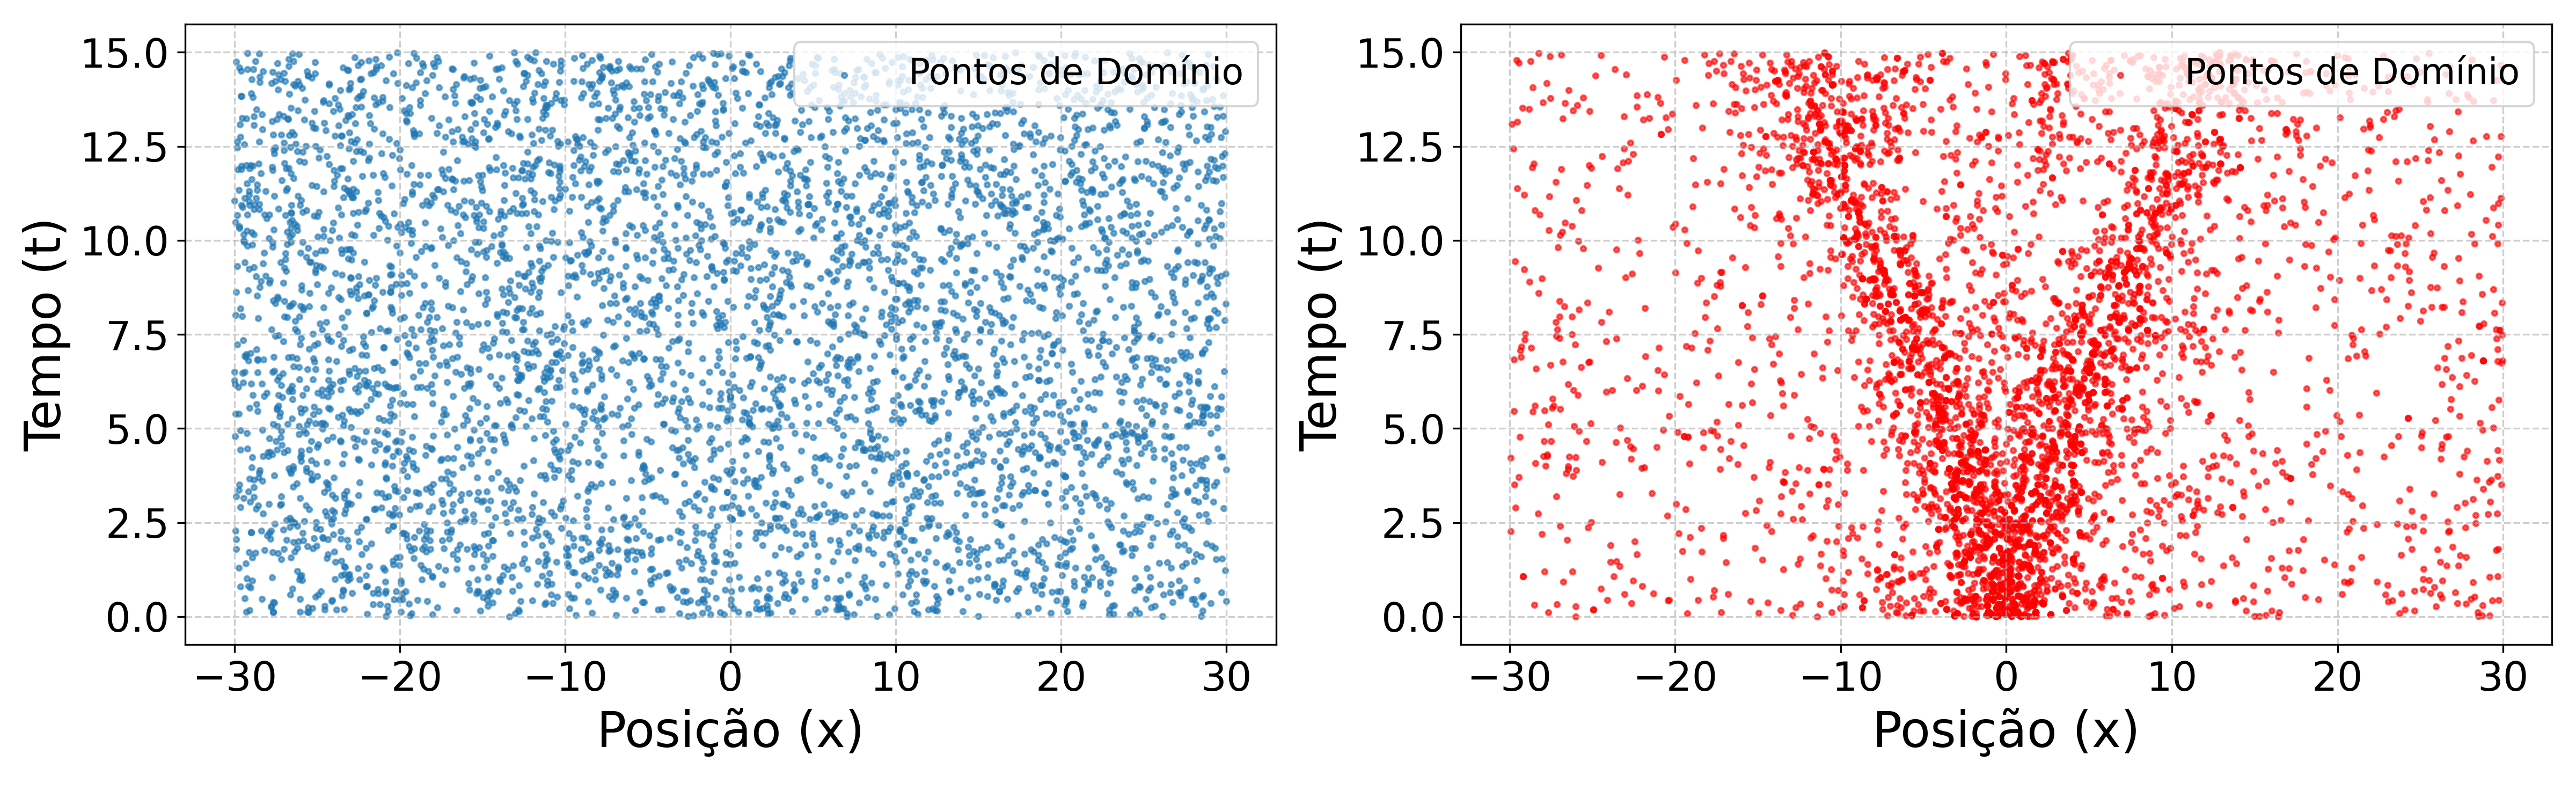
\includegraphics[width=\columnwidth]{imgs/rar_point_distribution_comparison.png}
        \caption{Distribuição de pontos: uniforme (esquerda) vs. adaptativa com RAR (direita).}        
        \label{fig:sampling_dist}
   \end{figure}

  \end{block}
\end{column}

\separatorcolumn

% --------------------
% --- COLUNA 2 -------
% --------------------
\begin{column}{\colwidth}
    \begin{block}{Resultados e Discussão}
        A PINN foi testada em cenários de complexidade crescente, porém ainda relativamente simples, com  $\alpha=\beta=10^{-4}$ e $\alpha=\beta=10^{-1}$ - regimes ainda pouco complexos, mas suficientes para observarmos alguns pontos importantes:
        \begin{figure}
            \centering
            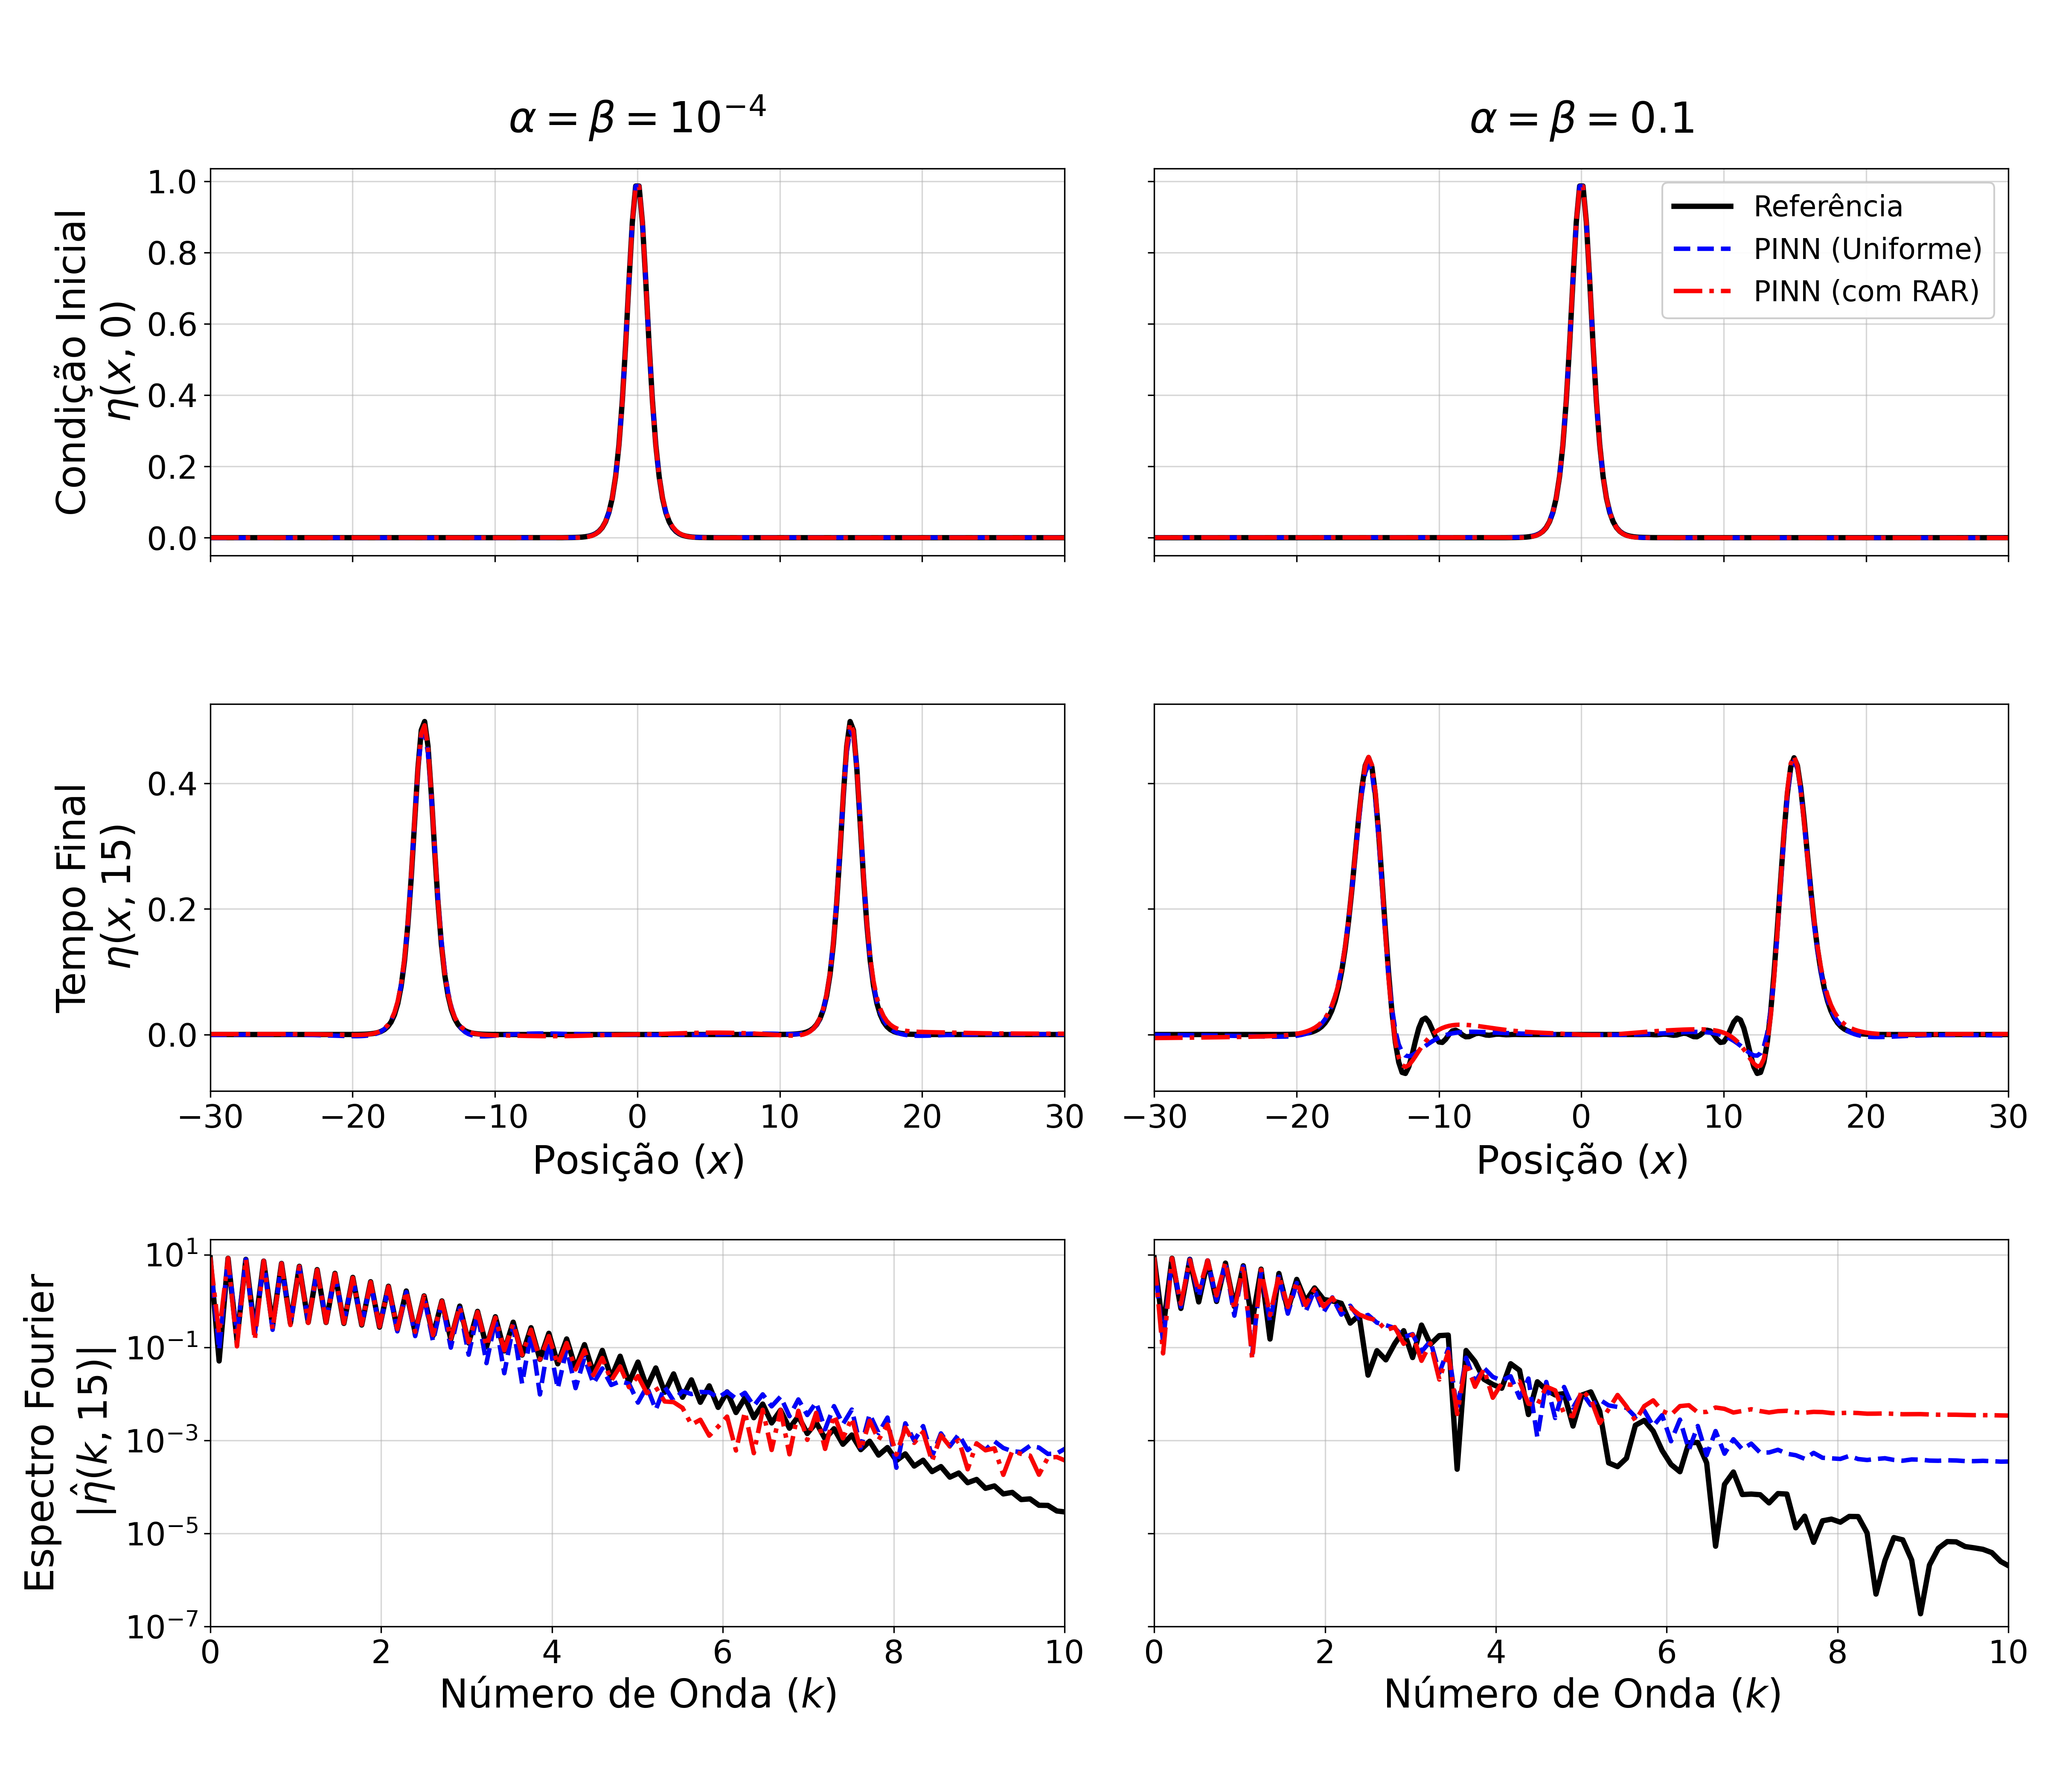
\includegraphics[width=\columnwidth]{imgs/boussinesq_panel_vertical.png}
            \caption{Comparação entre as soluções da PINN (Uniforme e com RAR) e a referência pseudo-espectral para os regimes de baixa ($\alpha=\beta=10^{-4}$, esquerda) e média complexidade ($\alpha=\beta=10^{-1}$, direita).}
            \label{fig:comparison}
        \end{figure}
        Conforme ilustrado na Figura \ref{fig:comparison}, no regime $\alpha=\beta=0.1$, a abordagem evidencia o Viés Espectral, mostrando que a PINN com amostragem uniforme (azul) possui mais dificuldade em aproximar. Já a PINN com estratégia RAR (vermelho) captura (mesmo sendo pouco) melhor as componentes de alta frequência, aproximando-se mais da solução de referência (preto), embora não elimine o efeito por completo.
    \end{block}

    \begin{block}{Conclusões}
        Este trabalho demonstrou que as PINNs possuem um desempenho de dupla face:
        \begin{itemize}
            \item São eficazes em regimes de baixa complexidade, onde os efeitos não lineares e dispersivos são suaves.
            \item Em regimes apenas um pouco mais complexos ($\alpha, \beta$ de ordem significativa), a performance é limitada pelo viés espectral e pela dificuldade da escolha de arquiteturas.
        \end{itemize}
        A amostragem adaptativa (RAR) se mostrou uma estratégia útil para mitigar este efeito, mas não o elimina por completo. Isso reforça que as PINNs são uma ferramenta emergente, e não uma substituta universal para métodos clássicos, necessitando de mais estudo sobre seus limites.
    \end{block}

    \begin{block}{Referências}
        \nocite{*}
        \bibliographystyle{plain}
        \bibliography{poster}
    \end{block}

\end{column}
\separatorcolumn
\end{columns}
\end{frame}

\end{document}